\documentclass{SMR}
\usepackage{paralist}
\usepackage{parallel}    % for side-by-side text (e.g. lyrics + translation)
\usepackage{polyglossia} % for foreign languages (foreign to the British, that is)
\usepackage{filecontents} % to illustrate citations

\begin{filecontents}{smr.bib}
 @book{1965smith_numerical_solution,
	title={Numerical Solution of Partial Differential Equations},
	author={Smith, G D},
	year={1965},
	publisher={Oxford University Press},
	location={London/New York},
}
\end{filecontents}


%graphics
\graphicspath{ {/Where/you/keep/your/graphics} }  % <- UPDATE THE PATH

%who and where
\smrtitle{SMR.cls}
\smrauthor{Marcin and Nick}
\smraffiliation{Edinburgh and Glasgow Universities}

\title{Scottish Music Review class file for XeLaTeX}
\author{Marcin Pietryszwski \and Nick Bailey}

\begin{document}

\newcommand{\cmd}[1]{\texttt{\textbackslash #1}}

\maketitle

\begin{abstract}
A class for the Scottish Music Review
\end{abstract}

\section{Section One} %section title comes here,

$\ldots$which you get by typing ``\cmd{section\{Section One\}}''
The usual title, author and date commands given in the preamble
are used to head up the paper, but there's also the smr- varients
which get used in the headers. 
If you don't supply them it'll still work, but you'll be warned.

If you supply an smrauthor, you \emph{must} supply an affiliation.

The title is set at the top left of left-hand pages, and the
author above the affiliation at the top right of right-hand pages.

To make this document, before
the \cmd{begin\{document\}} I said

\begin{verbatim}
\smrtitle{SMR.cls}
\smrauthor{Marcin and Nick}
\smraffiliation{Edinburgh and Glasgow Universities}

\title{Scottish Music Review class file for XeLaTeX}
\author{Pietryszwski, Marcin \and Bailey, Nick}
\end{verbatim}

\subsection{A Subsection} %subsections

Subsections are numbered per section. This one was obtained by saying
\cmd{subsection\{Subsection title\}}

\subsection{Text appearance}
Introduce emphasis like this: \cmd{emph\{Important\}}.
\emph{Important}: emphasis is a matter of house style.
We decide what it means.

%Footnotes\footnote{They break the flow and don't really
%mean anything in an on-line document; pages are for printing} are discouraged.
%Here is some text following a figure with a footnote added

Footnotes can be created with the \cmd{footnote\{\}} command, but we ask that
you format them as endnotes by putting
\begin{verbatim}
 \usepackage{endnotes}
 \let\footnote=\endnote
\end{verbatim}
in the preamble and \cmd{theendnotes} at the end of the document.

Only use single quotes, and type two get double ones. So
\verb!` - `` - ''-'! gives you ` - `` - ''-'. Mutiple dashes
give access to the different dashes use in properly-typeset documents
(that was one dash): 80--90\% (two) of people don't understand that
--- (three) why should they? The typesetter used to have to worry about that
in the old days.

\subsection{Figures in the text}

In \LaTeX, figures ``float'' (i.e. get placed where they look right).
It's best to use PDF files or PNG files, reserving JPEG files
for when there are actual photos. Otherewise there will be nasty artefacts.

Here is some text to be formatted followed by a figure of
a Klein Bottle as an example of how graphics are formatted
in this template.
\begin{figure}[h]
\caption{An included graphic. See how fuzzy it looks?}
\label{f:graphicexample} % Not before the caption!
\centering
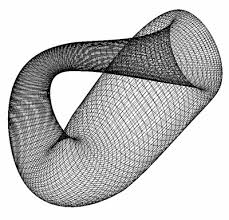
\includegraphics[width=0.5\textwidth]{klein.jpg}
\end{figure}

To get it I said
\begin{verbatim}
\begin{figure}[h]
\caption{An included graphic. See how fuzzy it looks?}
\label{f:graphicexample} % Not before the caption!
\centering
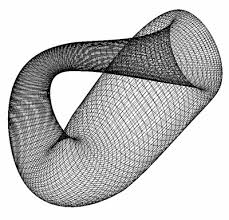
\includegraphics[width=0.5\textwidth]{klein.jpg}
\end{figure}
\end{verbatim}
which flagrently disregards what I said about JPEG diagrams, but there you go.

In particular, \emph{do not} use any raster format for musical score.
None of them play nice with the long horizontal lines on the staves
(because of science). Use Lilypond, or make a PDF and use that instead.

This example illustrated the optional argument in the sqaure brackets.
\texttt{h} means ``please think about putting the figure right here''.
The default for figures and tables is \texttt{htbf} (here, then top of the page,
then bottom of the page, then on a page by itself, in order of preference).

The \cmd{includegraphics[]\{\}} command takes the file name in curly brackets and
optional attributes in the square brackets.
The above example specifies the \texttt{width} of the figure as half that of the text.
Here's another example illustrating a few other attributes you can use when importing graphics:
\begin{figure}
 \caption{A Lorenz attractor}
 \label{f:lorenz}
 \centering
 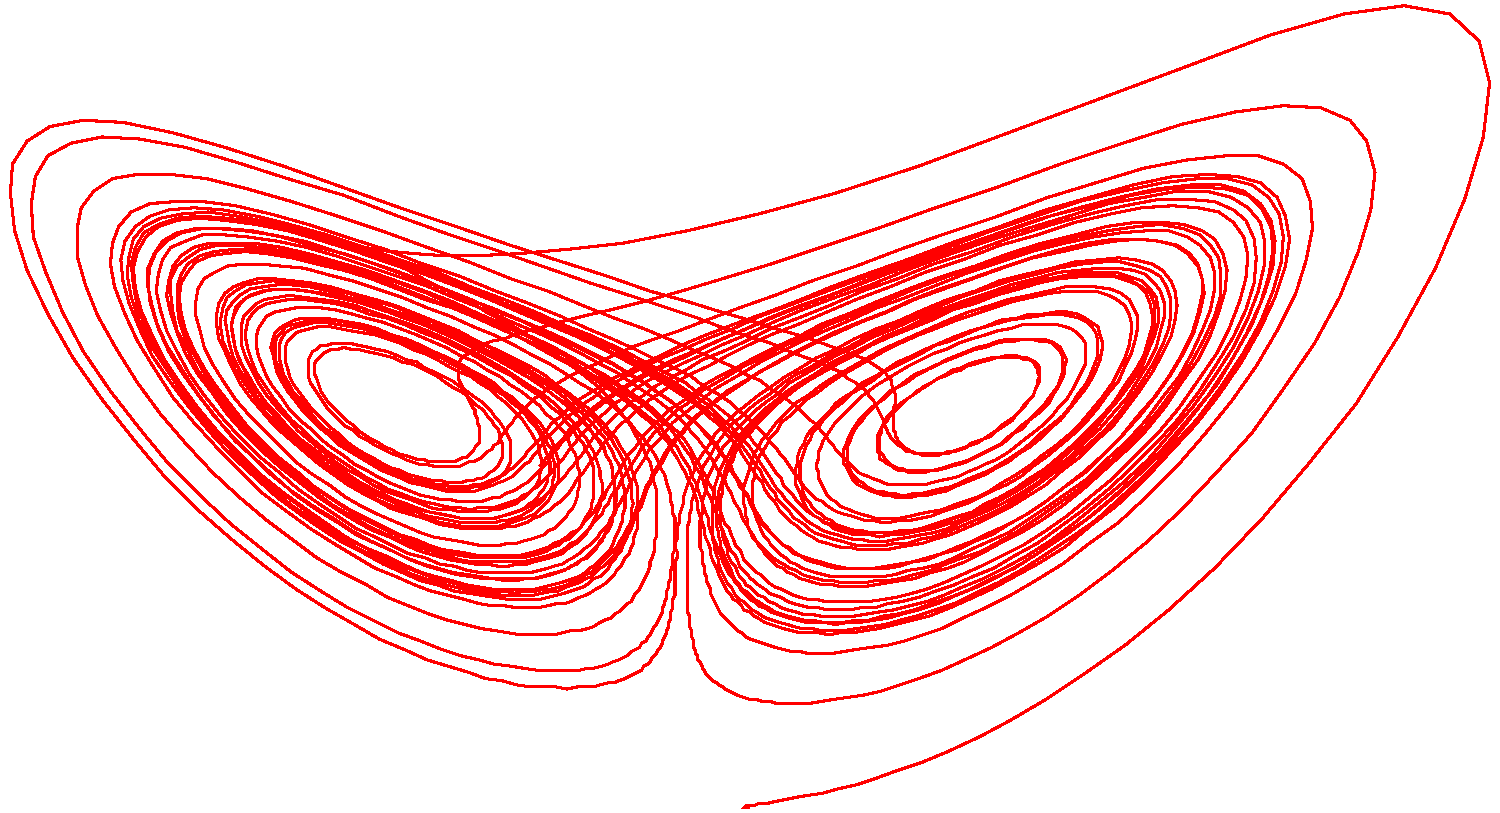
\includegraphics[scale=0.5, clip=true, trim=2cm 0 4cm 0]{Lorenz_Attractor_red}
\end{figure}
\begin{verbatim}
\begin{figure}
 \caption{A Lorenz attractor}
 \label{f:lorenz}
 \centering
 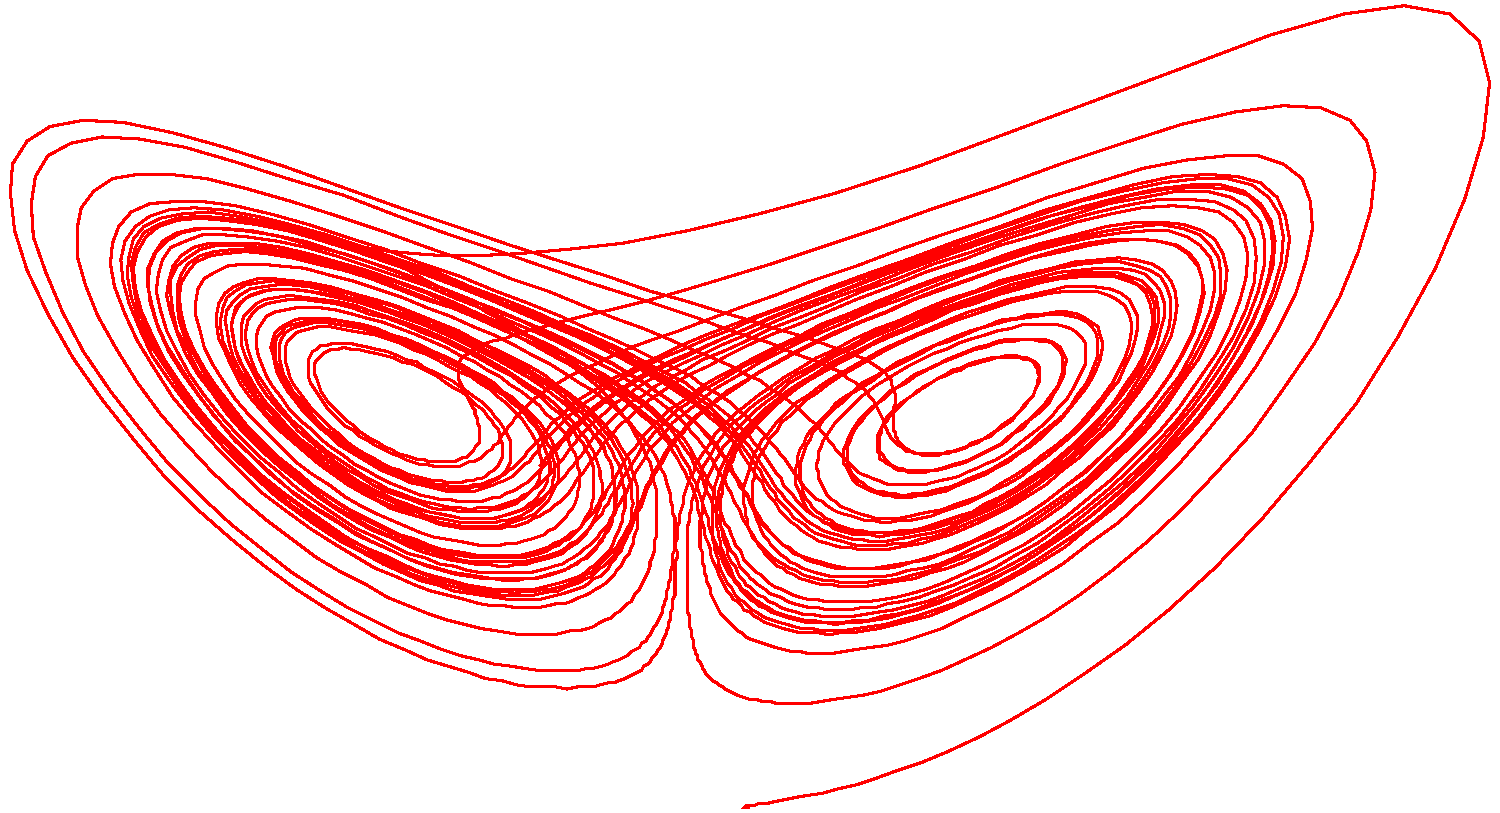
\includegraphics[scale=0.5, clip=true, trim=2cm 0 4cm 0]{Lorenz_Attractor_red}
\end{figure}
\end{verbatim}
If you want to crop the figure, use \texttt{trim=l b r t}, where the four lengths 
given specify the amount to trim off the left, bottom, right and top edges respectively. 
In order for this to work, you must also set \texttt{clip=true}. \texttt{scale} is 
self-explanatory and is only included to show more of the (many) possible attributes.


Never type something like \texttt{Figure 1} in your document.
Always label your figures with a unique name (I used \texttt{f:graphicexample};
the \texttt{f:} is my convention). Then refer to it in your text.
This way, you never get mis-numbered figures.

\begin{verbatim}
 Look at Figure~\ref{f:graphicexample}!
\end{verbatim}

Look at Figure~\ref{f:graphicexample}!
I also used the tilde, which makes sure there won't be a line-break between
the word and the number. You can also label sections, subsections etc
the same way.

\subsection{Citations}

\def\BibTeX{{\rm B\kern-.05em{\sc i\kern-.025em b}\kern-.08em
    T\kern-.1667em\lower.7ex\hbox{E}\kern-.125emX}}
Everybody either uses \BibTeX\ citations or can export them, so we shall not
describe that process here. To obtain the canonical form of a reference in
\BibTeX\ format, one might look it up on Google~Scholar which permits the \BibTeX
form to be copied to your computer's clipboard.

The SMR class defines the typesetting of the citations and the bibliography
using the \texttt{natbib} package, so if the \texttt{.bib} file contains

\begin{verbatim}
@book{1965smith_numerical_solution,
	title={Numerical Solution of Partial Differential Equations},
	author={Smith, G D},
	year={1965},
	publisher={Oxford University Press},
	location={London/New York},
}
\end{verbatim}

the correct form of citation can be obtained using \cmd{citep}
(parenthetised citation) like this:

\begin{verbatim}
PDEs can be fun~\citep{1965smith_numerical_solution}.
\end{verbatim}

PDEs can be fun~\citep{1965smith_numerical_solution}.

and saying \cmd{bibliography$\{$your\_bib\_file$\}$} at the place where
the bibliography should appear.

\bibliography{smr.bib}

\section{Heavy-duty usage}
\subsection{(Possibly multilingual) Side-by-Side Translations}
After saying \cmd{usepackage$\{$parallel$\}$} at the top of your document,
these can be achieved as follows:

\begin{verbatim}
 \begin{parallel}
  [<environment_options>]{<left-width>}{<right-width>}
\ParallelLText{<left-text>}
\ParallelRText{<right-text>}
\ParallelPar
\ParallelLText{<left-text>}
...
% The following <text> goes after the side-by-side text
% and before any footnotes...
\renewcommand{\ParallelAtEnd}{<text>}
\end{parallel}
\end{verbatim}

For example:

\setotherlanguage{greek}
\newfontfamily\greekfont[Script=Greek,Ligatures=TeX]{Linux Libertine O} % Has Greek characters
\begin{Parallel}[c]{}{} %Miss out the widths and it chooses for you; v = vertical line; p = page by page
 \ParallelRText{This is the Showing forth of the Inquiry of Herodotus of Halicarnassos,
 to the end that neither the deeds of men may be forgotten by lapse of time,
 nor the works great and marvellous, which have been produced some by Hellenes and
 some by Barbarians, may lose their renown; and especially that the causes may be
 remembered for which these waged war with one another.%
\footnote{Typeset using \url{https://www.ctan.org/pkg/parallel?lang=en}}}%
 \begin{greek}\ParallelLText{Ἡροδότου Ἁλικαρνησσέος ἱστορίης ἀπόδεξις ἥδε,
 ὡς μήτε τὰ γενόμενα ἐξ ἀνθρώπων τῷ χρόνῳ ἐξίτηλα γένηται,
 μήτε ἔργα μεγάλα τε καὶ θωμαστά, τὰ μὲν Ἕλλησι τὰ δὲ βαρβάροισι ἀποδεχθέντα, ἀκλεᾶ γένηται,
 τά τε ἄλλα καὶ δι᾽ ἣν αἰτίην ἐπολέμησαν ἀλλήλοισι.}\end{greek}%
 \ParallelPar
 \begin{greek}\ParallelLText{Περσέων μέν νυν οἱ λόγιοι Φοίνικας αἰτίους φασί γενέσθαι τῆς διαφορῆς.}\end{greek}
 \ParallelRText{Those of the Persians who have knowledge of history declare that the Phenicians first began the quarrel.}
 \renewcommand{\ParallelAtEnd}{With thanks to \url{http://www.sacred-texts.com/cla/hh/hh1000.htm}}
\end{Parallel}


\subsection{Music glyphs}
This style requires the lilyglyphs package (spelt
	\textit{lily}%
	\clefGInline[scale=0.8,raise=0.2]%
	\lilyOpticalSize{26}%
	ly\lilyDynamics{p}%
	\lilyOpticalSize{13}%
	\hspace*{0.2ex}\flat[scale=0.9,raise=0.2]%
	\lilyOpticalSize{11}%
	\lilyDynamics{s}) which
enables the use of Lilyponds Emmentaler font in the text. The full documentation
is available on
\href{http://mirrors.ctan.org/macros/luatex/latex/lilyglyphs/documentation/lilyglyphs.pdf}{CTAN}.
Glyphs are included through their names, and most are guessable, but a necessarily abbreviated
crib sheet follows.

\begin{table*}
{\small
\begin{tabular}{r|l l}
\wholeNote & \cmd{semibreve} -- \cmd{wholeNote}\\
\wholeNoteDotted & \cmd{semibreveDotted} -- \cmd{wholeNoteDotted}\\
\halfNote & \cmd{minim} -- \cmd{halfNote}\\
\halfNoteDown & \cmd{minimDown} -- \cmd{halfNoteDown}\\
\halfNoteDotted & \cmd{minimDotted} -- \cmd{halfNoteDotted}\\
\halfNoteDottedDown & \cmd{minimDottedDown} -- \cmd{halfNoteDottedDown}\\
\halfNoteDottedDouble & \cmd{minimDottedDouble} -- \cmd{halfNoteDottedDouble}\\
\halfNoteDottedDoubleDown & \cmd{minimDottedDoubleDown} -- \cmd{halfNoteDottedDoubleDown}\\
\crotchet & \cmd{crotchet} -- \cmd{quarterNote}\\
\crotchetDown & \cmd{crotchetDown} -- \cmd{quarterNoteDown} & etc...\\
\quaver & \cmd{quaver} -- \cmd{eighthNote}\\
\quaverDown & \cmd{quaverDown} -- \cmd{eighthNoteDown} & etc...\\
\semiquaver & \cmd{semiquaver} -- \cmd{sixteenthNote}\\
\semiquaverDown & \cmd{semiquaverDown} -- \cmd{sixteenthNoteDown}\\
\demisemiquaver & \cmd{demisemiquaver} -- \cmd{thirtysecondNote}\\
\demisemiquaverDown & \cmd{demisemiquaverDown} -- \cmd{thirtysecondNoteDown}\\
\threeBeamedQuavers & \cmd{threeBeamedQuavers} & Three beamed quavers\\
\threeBeamedQuaversI & \cmd{threeBeamedQuaversI} & Second dotted\\
\threeBeamedQuaversII & \cmd{threeBeamedQuaversII} & First dotted\\
\threeBeamedQuaversIII & \cmd{threeBeamedQuaversIII} & Second dotted, first short\\
\hline
\clefGInline & \cmd{clefG}, \cmd{clefGInline} & clefs.G\\
\clefFInline & \cmd{clefF}, \cmd{clefFInline} & clefs.F\\
\clefCInline & \cmd{clefC}, \cmd{clefCInline} & clefs.C\\
\hline
\lilyTimeC & \cmd{lilyTimeC} & timesig.C44\\
\lilyTimeCHalf & \cmd{lilyTimeCHalf} & timesig.C22\\
\lilyTimeSignature{7}{8} & \cmd{lilyTimeSignature\{7\}\{8\}}\\
\lilyTimeSignature{3 + 4}{4 + 8} & \cmd{lilyTimeSignature\{3 + 4\}\{4 + 8\}}\\
\hline
\natural & \cmd{natural} & accidentals.natural\\
\sharp & \cmd{sharp} & accidentals.sharp\\
\flat & \cmd{flat} & accidentals.flat\\
\flatflat & \cmd{flatflat} & accidentals.flatflat\\
\hline
\wholeNoteRest & \cmd{wholeNoteRest} & Whole Note Rest\\
\wholeNoteRestDotted & \cmd{wholeNoteRestDotted} & DottedWhole Note Rest\\
\halfNoteRest & \cmd{halfNoteRest} & Half Note Rest\\
\halfNoteRestDotted & \cmd{halfNoteRestDotted} & Dotted Half Note Rest\\
	\halfNoteRestDotted\lilyPrintMoreDots & 
	\cmd{halfNoteRestDotted}\cmd{lilyPrintMoreDots} &
	Example of Double Dotted Rest\\
\crotchetRest & \cmd{crotchetRest} & Crotchet Rest\\
\crotchetRestDotted & \cmd{crotchetRestDotted} & Dotted Crotchet Rest\\
\quaverRest & \cmd{quaverRest} & Quaver Rest\\
\quaverRestDotted & \cmd{quaverRestDotted} & Dotted Quaver Rest\\
\semiquaverRest & \cmd{semiquaverRest} & Semiquaver Rest\\
\semiquaverRestDotted & \cmd{semiquaverRestDotted} & Dotted Semiquaver Rest\\
\hline
\lilyDynamics{f} & \cmd{lilyDynamics\{f\}} & forte\\
\lilyDynamics{p} & \cmd{lilyDynamics\{p\}} & piano\\
\lilyDynamics{m} & \cmd{lilyDynamics\{m\}} & mezzo-\\
\lilyDynamics{r} & \cmd{lilyDynamics\{r\}} & rin-\\
\lilyDynamics{s} & \cmd{lilyDynamics\{s\}} & s-\\
\lilyDynamics{z} & \cmd{lilyDynamics\{z\}} & -z\\
\end{tabular}
}
\caption{Get-you-started-quick crib sheet for music glyphs in the body text}
\end{table*}




\end{document}
